\documentclass[tikz,border=5pt]{standalone}
\usepackage[UTF8]{ctex}
\usepackage{amsmath,amssymb}
\usetikzlibrary{arrows.meta,calc,angles,quotes,decorations.pathmorphing,patterns}
\definecolor{ink}{HTML}{243447}\definecolor{blue}{HTML}{2765A2}
\definecolor{green}{HTML}{3F7D5B}\definecolor{red}{HTML}{B74739}
\tikzset{body/.style={draw=ink,thick},vec/.style={draw=blue,thick,-{Latex}},guide/.style={gray!65,dashed},dim/.style={ink,{Latex}-{Latex}},line cap=round,line join=round}
\begin{document}

\begin{tikzpicture}
\draw[gray](-4,0)--(4.5,0);
\draw[blue,thick,{Latex}-{Latex}](0,-1.4)--(0,1.4);
\node[above]at(0,1.4){透镜};
\draw[body](2,-1.3)to[bend left=15](2,1.3);
\foreach \y in {-1.15,-.9,...,1.15}\draw[gray](2.18,\y)--++(.22,.15);
\draw[vec](2,1.7)--(3.4,1.7)node[midway,above]{$v$};
\draw[body,-{Latex}](-1.9,0)--(-1.9,.8)node[above]{物};
\draw[body,-{Latex}](-3.2,0)--(-3.2,-.8)node[below]{像};
\draw[dim](-3.2,-1.7)--(0,-1.7)node[midway,below]{$2f$};
\draw[dim](-1.9,1.2)--(0,1.2)node[midway,above]{$x(t)$};
\draw[vec](-.2,.35)--(-3.7,.35)node[left]{$x$};
\node[below right]at(0,0){$0$};
\draw[dim](0,-.7)--(2,-.7)node[midway,below]{$d=vt$};
\end{tikzpicture}
\begin{tikzpicture}
\draw[gray,-{Latex}](-4.2,0)--(4.5,0)node[right]{$X$};
\draw[blue,thick,{Latex}-{Latex}](0,-.9)--(0,2.7);
\draw[body](1.5,-.9)to[bend left=15](1.5,1.5);
\foreach \x/\lab in {-3/Y,-1/{-x},1.5/d,3/a}{\fill[ink](\x,0)circle(.035);\node[below]at(\x,-.1){$\lab$};}
\draw[blue,thick](-1,0)--(0,.8)--(1.5,1.2);
\draw[guide](-3,0)--(0,.8);
\draw[green,thick,-{Latex}](1.5,1.2)--(0,2.4)--(-3,0);
\draw[green,dashed](1.5,1.2)--(3,0);
\node[above]at(-2.7,.85){第一次的虚像};
\node[above]at(3,.4){反射后的等效物};
\draw[dim](0,-.75)--(1.5,-.75)node[midway,below]{$d$};
\node at(0,-1.6){示意位置：$d=f,\;Y=-2f,\;a=2f$};
\end{tikzpicture}
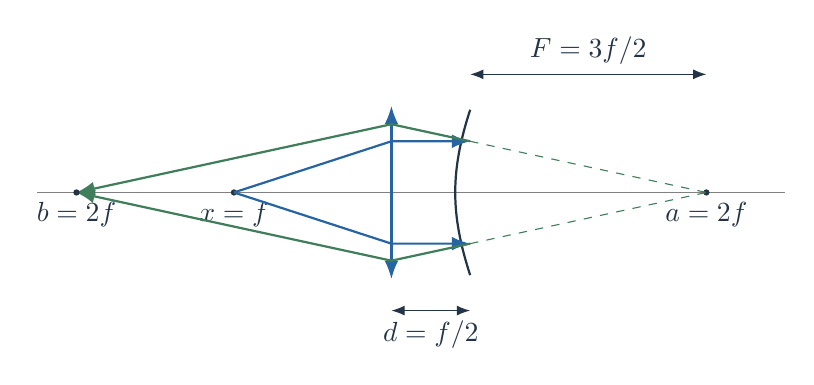
\begin{tikzpicture}
\draw[gray](-4.5,0)--(5,0);
\draw[blue,thick,{Latex}-{Latex}](0,-1.1)--(0,1.1);
\draw[body](1,-1.05)to[bend left=18](1,1.05);
\fill[ink](-2,0)circle(.04)node[below]{$x=f$};
\fill[ink](4,0)circle(.04)node[below]{$a=2f$};
\foreach \h in {-.65,.65}{
\draw[blue,thick,-{Latex}](-2,0)--(0,\h)--(1,\h);
\draw[green,thick,-{Latex}](1,\h)--(0,{4*\h/3})--(-4,0);
\draw[green,dashed](1,\h)--(4,0);}
\fill[ink](-4,0)circle(.04)node[below]{$b=2f$};
\draw[dim](0,-1.5)--(1,-1.5)node[midway,below]{$d=f/2$};
\draw[dim](1,1.5)--(4,1.5)node[midway,above]{$F=3f/2$};
\end{tikzpicture}
\begin{tikzpicture}
\draw[vec](0,0)--(7.5,0)node[right]{$u=vt/f$};
\draw[vec](0,-2.5)--(0,3.8)node[above]{$x/f$};
\draw[guide](0,1)--(7.2,1)node[right]{$1$};
\draw[guide](3.162,-2.4)--(3.162,3.6)node[above,text=ink]{$u_{\rm D}$};
\draw[blue,thick,domain=0:1.303,samples=80]plot({2*\x},{(\x*\x+\x-3)/(\x*\x-2.5)});
\draw[red,thick,domain=1.303:1.475,samples=70]plot({2*\x},{(\x*\x+\x-3)/(\x*\x-2.5)});
\draw[blue,thick,domain=1.78:3.5,samples=90]plot({2*\x},{(\x*\x+\x-3)/(\x*\x-2.5)});
\fill[blue](0,1.2)circle(.035)node[left]{$6/5$};
\fill[white,draw=ink](2.606,0)circle(.045)node[above left,text=ink]{$u_{\rm N}$};
\node[red]at(2.4,-2.1){$x<0$};
\node[blue]at(5.7,2.6){有限正物距};
\node[blue]at(.95,2.1){有限正物距};
\end{tikzpicture}
\end{document}
